\section{Background and Related Work}

\subsection{Centralized Data Fusion}

% Talk about standard centralized fusion approaches.
% Algorithms such as EKF, etc. networking setup.

The most common approach for SDA tracking applications is a centralized approach. 
In this approach, measurements from a common region or satellite are sent to a ground station where a powerful computer is able to run state of the art data fusion algorithms.
This allows the highest quality filters to be ran on the data, allowing for super high fidelity tracking. 
Additionally, the algorthimic approach is quite simple and easy to implement, imagine just a single Extended Kalman Filter (EKF) \cite{b5} running a batch update on hundreds of measurements all at the same time.
This approach also allows easy communication protocols for satellites on where they should send their measurements too; you just always send it to the centralized ground station.

The centralized architecture was primarily designed around a human operator. With a centralized location for all data management and fusion, an operator can easily monitor the system and make decisions.
Some decisions an operator might make would be which friendly assets should recieve certain data about an enemy target, where should the sensors on the satellites be pointed, and which areas of the globe should be given a higher priority.

However, there are several negative aspects to this approach. First, the system has a critical point of failure. All measurements and tracks exist and are processed at a single point,
which means if that point is compromise the whole system fails. Additionally, the system has a large amount of inertia in decision making and processing. Waiting for a human operator to make a decision can cost time which is extremely valuable in a warfighting environment.
Also, when critical information needs to be sent to friendly assets, that data first has to be sent from satellite to ground station for processing, then from ground station back to a communication satellite that can relay the information to the reqeusting asset.

\subsection{Decentralized Data Fusion}

An alternative approach to centralized data fusion is decentralized data fusion (DDF). In DDF, individual agents run their own estimation algorithms on the data they collect or recieve.
Then, collabratively, these agents communicate with each other to reconsile their information into a better single estimate. DDF is widely used in multi-agent systems where agents are able to sense, communicate, and process information \cite{b1}.

\begin{figure}[h]
    \centering
    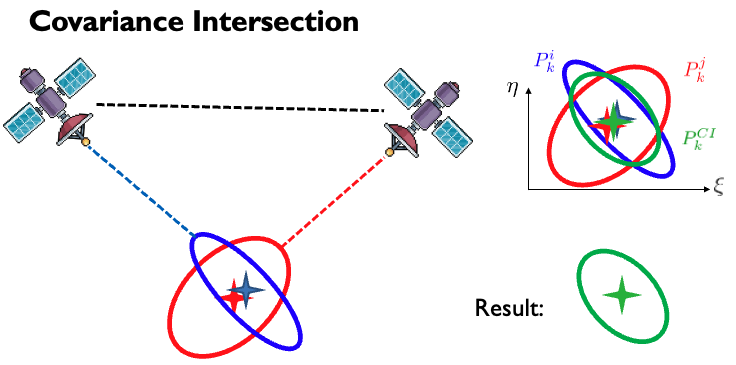
\includegraphics[width=0.35\textwidth]{figs/covariance_intersection.png}
    \caption{Covariance Intersection Fusion to combine two mono tracks into a fused track. The blue and red ellipses are the covariance of the two estimates. The green ellipse is the resulting covariance of the fused estimate. }
    \label{fig:ci_fusion}
\end{figure}

In the context of SDA applications, DDF may be useful for tracking ground targets. If each satellite was intelligent enough to run its own onboard estimation algorithm, such as an EKF,
then the satellites could communicate with each other to reconsile their information into a better single estimate.
This is particularly useful for satellites as measurements taken by satellite sensors are typically bearings only measurements. 
A bearings only measurement is just a line of sight vector from a satellite to a location in the sensor frame.
By itself, a bearings only measurement is not enough to estimate a 3D position as there is a missing dimension, but, when combined with multiple measurements, especially from different viewing angles, the 3D position can be reconstructed.
In the satellite tracking context this is known as upgrading a track from a mono-track to a stereo-track, giving it multiple dimensions of information.
The DDF algorithm covariance intersection (CI), shown in Figure~\ref{fig:ci_fusion}, is a widely used algorithm that employs this strategy and has been the state of the art for DDF applications for over 25 years \cite{b4}. 

If the DDF approach was implemented in a satellite network, it would allow for much more robust tracking and agile decision making. By decentralizing the data and information, you remove the critical point of failure in the system. 
Also, if the critical information is processed in the sky user requests for data can be quickly transmitted, instead of having to go back and forth with a ground station system.


% Talk about decentralized fusion approaches.
% Algorithms such as covariance intersection and et-ddf.
% How these approaches are used in the cooperative tracking domain.

